\documentclass[%
%sor,
%aip,
aps,
draft, % doesn't print figures, among others. Compiles faster
%final, % removes todos
%twoside,
%groupedaddress,
jmp,
 jor,
 amsmath,amssymb,
%preprint,%
 reprint,%
%author-year,%
%author-numerical,%
]{revtex4-2}

\usepackage{graphicx}% Include figure files
\usepackage{dcolumn}% Align table columns on decimal point
\usepackage{bm}% bold math
%\usepackage[mathlines]{lineno}% Enable numbering of text and display math
%\linenumbers\relax % Commence numbering lines

\usepackage[obeyFinal,%
]{todonotes} 
\newcommand{\TODO}[1]{\todo[inline]{TODO: #1}} % creates new command, \TODO. The ordinary, non-inline, version of \todo doesn't work well with the columns (especially longer todos). 
\newcommand{\note}[1]{\todo[inline]{#1}} % creates new command, \TODO. The ordinary, non-inline, version of \todo doesn't work well with the columns (especially longer todos). 

\begin{document}
\title[Sample title]{Efficient area coverage with random search}%\footnote{Error!}}% Force line breaks with \\
%\thanks{Very rough draft.}


\author{Marko Guberina}
\author{Christian Josefson}%

\author{Anders Segerlund}
\affiliation{%
Chalmers University of Technology%\\This line break forced% with \\
}%

% some other stuff we can include if we want
 %\homepage{http://www.Second.institution.edu/~Charlie.Author.}
 %\altaffiliation[Also at ]{Physics Department, XYZ University.}%Lines break automatically or can be forced with \\
 %\email{Second.Author@institution.edu.}
%\affiliation{ 
%Chalmers University of Technology%\\This line break forced with \textbackslash\textbackslash
%}%

\date{\today}% It is always \today, today,
             %  but any date may be explicitly specified

\begin{abstract}
%An article usually includes an abstract, a concise summary of the work
%covered at length in the main body of the article. It is used for
%secondary publications and for information retrieval purposes. 
An abstract of the paper. Will be done last.
%
\listoftodos
\end{abstract}

\keywords{Suggested keywords}%Use showkeys class option if keyword
                              %display desired
\maketitle


%% Assignment text: 
% The report should be written in RevTex 4.2 (see https://journals.aps.org/revtex (Links to an external site.)), using the format of Physical Review X with a limit of 8 pages in double-column reprint format (including pictures and references). If needed, you can have an extra document containing an unlimited amount of Supplementary Materials.

% Structure your report like a scientific article, with an abstract summarising the rationale and results of the project; an introduction shortly explaining its background and motivating why the question is interesting; methods and/or results section(s) describing your model and what you do with it; a discussion section; and ending with a conclusion. Put some work into the discussion and conclusion sections. This is where you demonstrate that you truly understand the implications of your work, including shortcomings and uncertainties. It is important that the discussion does not fall out as a simple summary of what the figures show.



\section{Introduction}
This project explores the usage of random search algorithms in swarm robotics.
We first introduce the concept of swarm robotics. 
Many robotics applications call for usage of multiple robots, search being one of them, as it
clearly it is easier to find desired targets if there are multiple agents performing the search operation.
The term swarm robotics denotes the case when there are many robotic agents which when working together
exhibit collective (group) behaviour.
These robots are typically very simple and their operation is often inspired by animals such 
as ants or bees.
The benefits of using a large number of simple robots rather than a few more capable and complex robots
are the following:
\begin{itemize}
		\item price -- such robots are very cheap to produce as they require just the basic of-the-shelf components
		\item robustness -- failure of a single robot has a small impact on the overall result
		\item scalability -- swarms are designed to handle a very large number of agents and new agents
				can very easily be introduced as the swarm is typically controled in a distributed fashion
		\item equally complex results 
				-- even through the robots themselves are simple, they can produce complex
				emergent behaviours and are thus very adaptable
\end{itemize}
Some of the above points need to be elaborated further. 
Robustness is achieved by having all robots identical in both form and function which
makes them mutually interchangable. 
Having indentical robots also makes it easy to simply add more robots.
However, additional care in algorithm design is required to avoid diminishing returns
when adding new robots. Of course, at some point cluttering will prevent robots from moving,
but we aim to achieve the full potential of the swarm.
Achieving equally complex results is the key feature which needs to be delivered. 
In essence, this means that we should view the swarm as a single ``distributed robot''
which makes intelligent decisions to obtain the desired result. In other words,
the swarm needs to feature collective emergent behaviour which makes it better
than the sum of its parts, just like ants or bees.

Now let us address the problem we wish to solve:
achieving efficient autonomous search in unknown and/or changing environments.
How a search problem is solved critically depends on a few factors:
existance of a map and the ability of robots to localize themselves in the map.
Clearly, if the robots know where they are and where they could go, classic search
algorithms like A* would deliver provably optimal results.
However, many environments are not (accuratelly) mapped, like forests or ocean floors,
or they change over time. Furthermore, to localize robots must use GPS or
have known landmarks from which they can estimate their position.
This is so because odometry (starting from a known position and 
then integrating velocity (which is locally known)) very quickly accumulates errors which makes it 
unusable for all but short paths.
In this project we deal with unknown GPS denied environments.

Before proceeding to our solution, we need to discuss another important problem:
coordination. In order to use deterministic coordination algorithms, the robots
need to communicate. Given the environments we are interested in, robots would need to
endowed with powerful radio antenas to communicate with a global central node and
that would overall be very impractical. 
Thus the only communication option in this case would be local communication between neighbouring robots.
In the current implementation of the project this is not used, but there are situations in which
it would be useful, for example to signal presence of multiple found targets.
This is left as future work.



The above leads us to the following solution: using random walks as search algorithms.
This choise is in line with our design desires because it takes very little computational
power to implement these algorithms and that enables us to have (very) small and low powered robots.
One type of random walks are Levy walks. The idea is inspired by nature as 
this type of walk can be can be observed in hunting paterns of many different types of animals.
More importantly, we can mathematically show that this leads to higher area coverage efficiency 
in an obstacle free environment when compared to other types of random walks.
However, the situation is much more complicated in environments with obstacles. Namely, because
the obstacles prevent the free movement of robots, the possible and the resulting walking patterns will 
be different. 
Furthermore, the robots must not colide with obstacles or other robots. Even with more lax
collision requirements, they should at least
avoid them to prevent getting stuck. To combat this problem, artificial potential fields are employed.
In essence this just means that robots are repelled from obstacles each other by some amount.
Another benefit of artificial potential fields in this case is that they help with diffusion of
robots accross the environment. Given the role of artificial potential fields in this project, 
they are manually defined to satisfy the collision avoidance requirement.
These new complications introduced by obstacles lead us to our research questions:

\begin{enumerate}
\item How do different types of random search algorihms perform in different types of environments?
\item Will switching and dynamic tuning of the random search algorihms produce better results?
\end{enumerate}

The rest of this project report is organized as follows: first we mathematically define 
the random walks. We then introduce the environments we are interested in and 
explain our usage of artificial potential fields.
Next we present the derived robot control algorithms show their performance accross different 
environments. Finally we provide a discussion of the results and the summary of our findings.



There are a multitude of scenarios which consist of a search through unknown environments; some examples are: search and rescue in a burning building, searching for wildfires in a forest, trash collection (urban and in nature), mapping indoor environments and search for pollution. \TODO{Find references}

%\begin{itemize}
%\item Finding wildfires
%\item Searching for people
%\item Finding and picking up trash
%\item Mapping indoor environments
%\item Data collection in complex environments
%  \begin{itemize}
%  \item Fish population in oceans
%  \item Pollution
%  \end{itemize} 
%\end{itemize} 

\TODO{Paragraphs briefly explaining brownian motion, active brownian motion and Levy flights. Not very math-y, yet; we'll go into the proper theory in Methods. Just ``Brownian motion is a kind of random motion, used to model the random motion of particles, and was developed by Einstein back in the day'' etc.}


\section{Methods}

\subsection{Comparison of different random walks}
Three types of walks: Brownian motion, active brownian motion and Levy flights.\TODO{can we call brownian motion and active brownian motion different types of walks? We can, right?} \note{\cite{basu2018active} talks a bit about how Active brownian motion is similar to brownian motion on a very long timescale, but initially it is very different. Maybe that's worth mentioning? (See section II. Model)}

\subsection{Simulation}
In order to answear our research question, we developed a 2D simulation.
The simulation contains three types of objects: {\em agents (robots)}, {\em targets} and {\em obstacles}. 
The agents are the only active objects; they diffuse throughout the surrounding area, searching for items. 
The agents all have a radius within which they can see, which will be called a visibility sphere. 
For simplicity, all sensors have the same visibility sphere radius.
The items can represent different things: wildfires, people (during search and rescue), pollution etc. 
The obstacles are hindrances that the agents have to move around, for example trees and streetlights. 

Using an agent-based model several different types of random walks will be explored. Eventually, the agents will be given the capability to switch between different types of walks depending on their experience with the surrounding environment, for example if a robot has had little success with finding items the last couple of timesteps it switches to a walk type more effective in sparse environments.  \TODO{Make sure we actually switch between walks!}
The hope is that this will lead to better results in random environments than using any of walk types by themselves.


As the impact of the geometry of the objects was not under evaluation all of the objects are represented by circles. \note{Write anything more about the geometry?} 

% We want the search to consist of both a random component and something which directs it towards the items, but without swarming at one item. What we ended up doing was Levy flights together with an artificial potential field.\todo{Right? } 

%Define brownian motion and Levy flights, mention when they are best utilized.
\subsection{Artificial potential field}
There are currently no ways to ensure that the agents avoid collisions, both with each other and with obstacles. During simulation, the agents can pass through each other without problem, but in real life situations we need to avoid collisions to avoid damage. \note{Feels kinda stupid to note that we want to avoid collisions, but on the other hand I feel like stuff like that is nice to mention?}

One remedy to keep them from colliding is to imbue the agents and obstacles with artificial potential fields, which repulses them from each other, with the strength of the repulsion increasing as the distance between the objects decreases. 
% inverse proportionally? Inverse square? 





\subsection{Optimizing parameters with a genetic algorithm} 
TBD. Have the algorithm, need to figure out how to run it with the simulation. 

\section{Results}
Intuitively the robots seem to move as expected, no walking just past items they should try to pick up etc. Need to quantify this though. 


\begin{figure}
    \centering
    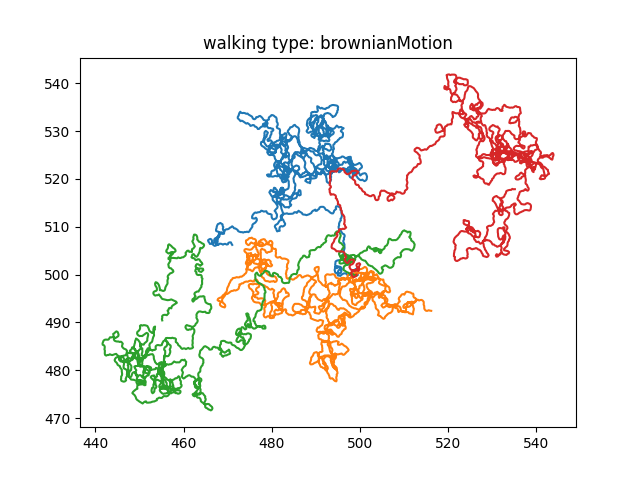
\includegraphics[width=\columnwidth]{figures/brownianMotion.png}
    \caption{Figure testing. Brownian motion picture}
    \label{fig:my_label}
\end{figure}
\section{Discussion}

Proposal of things to mention: 
\begin{itemize}
    \item How the switching works (well or not well?) 
    \item With and without artificial potential fields
    \item Artificial potential fields on the items
    \item Optimization (if we do that)
    \item Impact of different geometries? 
    \item Compare results to similar studies? 
\end{itemize}



\bibliography{refs.bib}
\end{document}